\documentclass{standalone}
\usepackage{tikz}
\usetikzlibrary{patterns, positioning}
\usepackage[sfdefault]{ClearSans} %% option 'sfdefault' activates Clear Sans as the default text font
\usepackage[T1]{fontenc}

\begin{document}
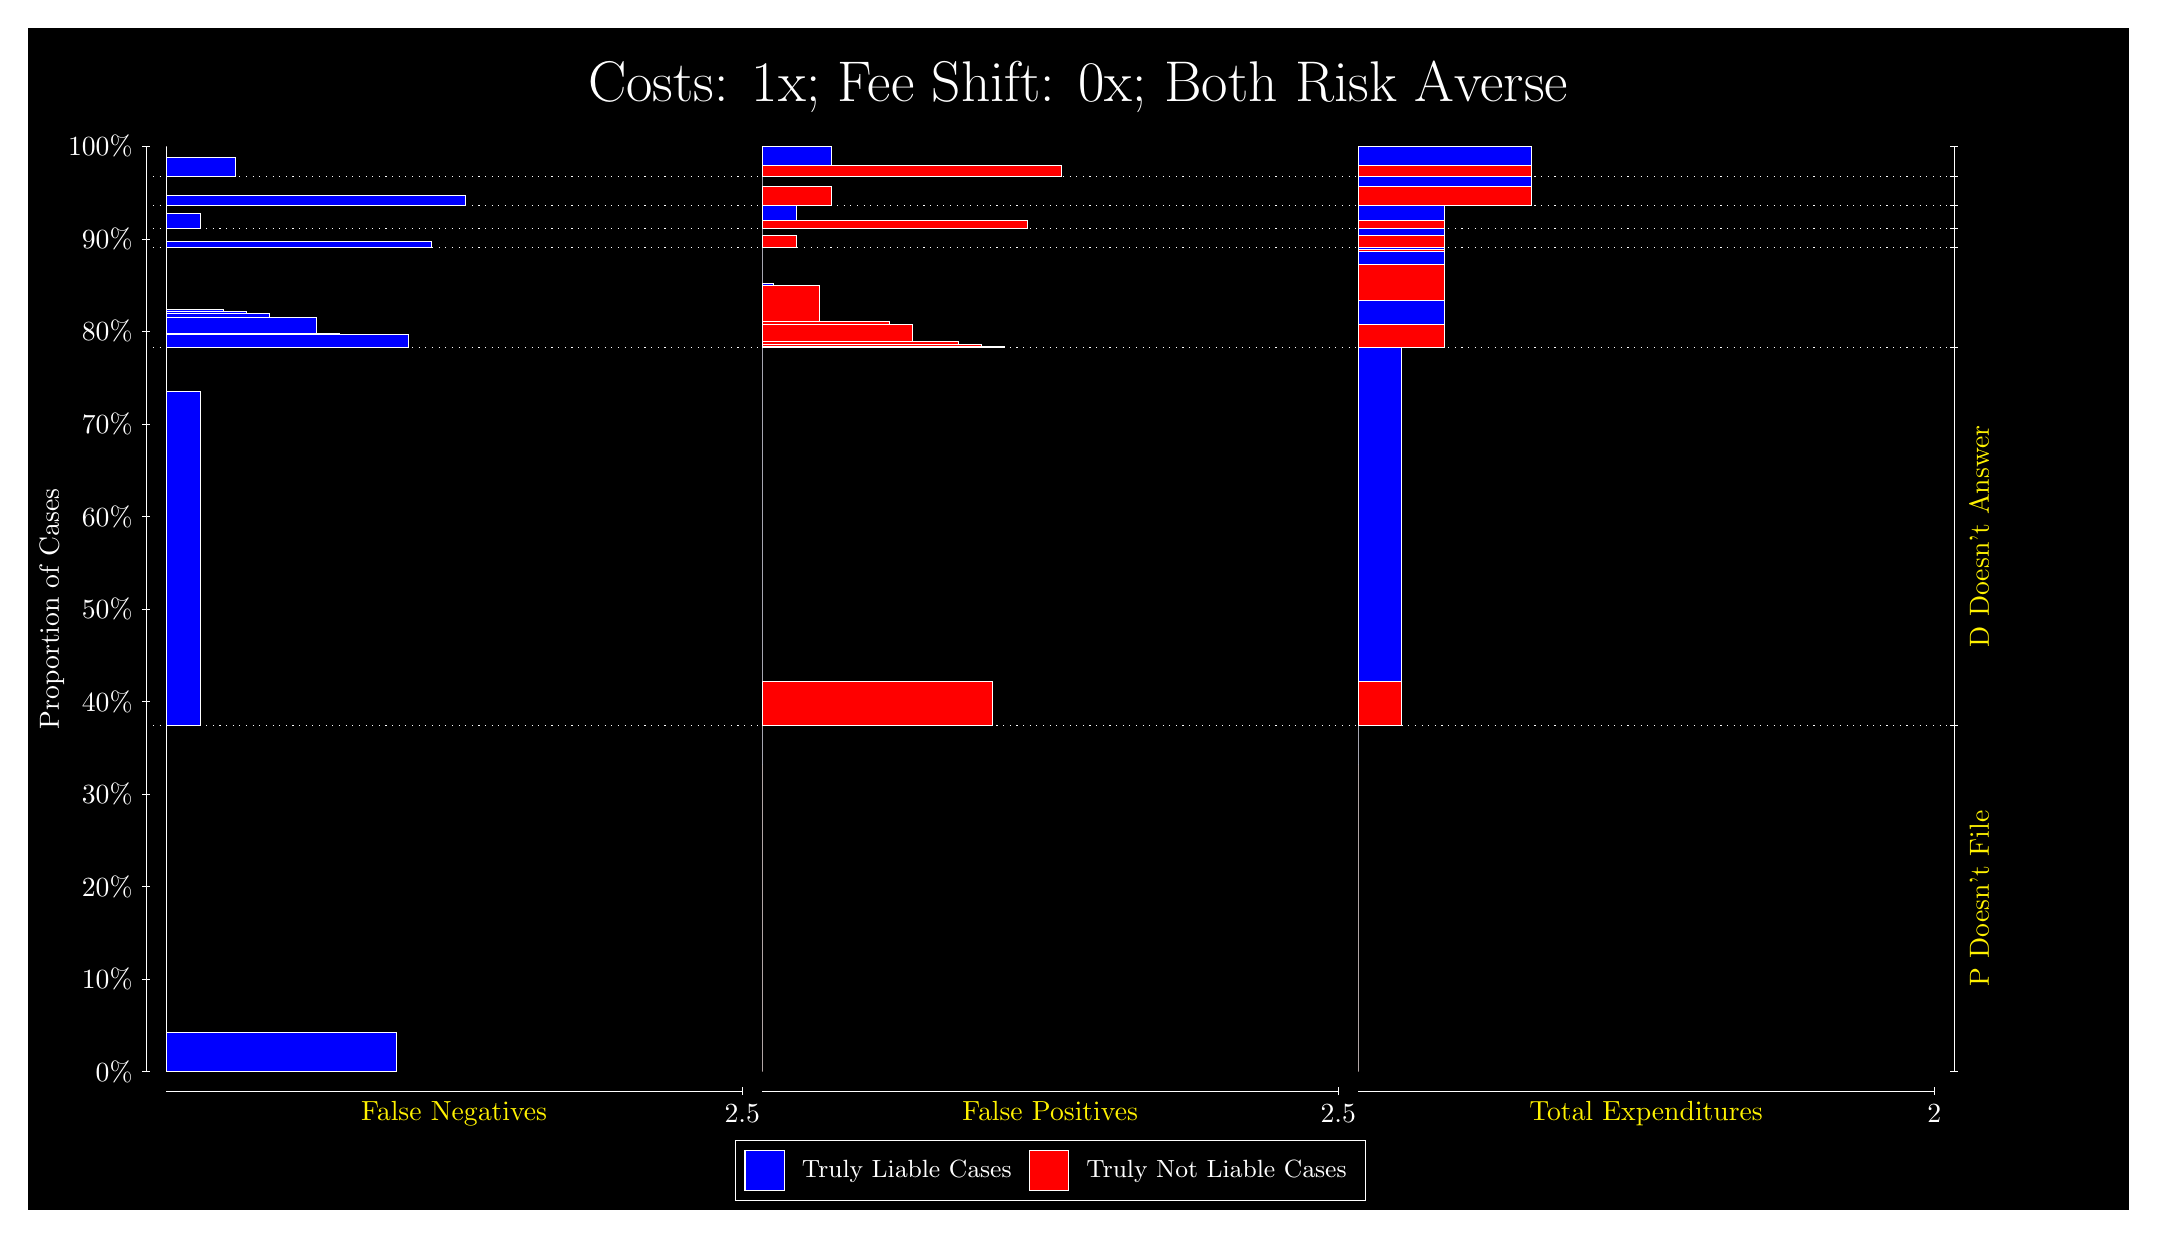
\begin{tikzpicture}
\draw[fill=black] (0,0) rectangle (26.667,15);
\draw[text=white] (0,13.5) rectangle (26.667,15) node[midway] {\huge Costs: 1x; Fee Shift: 0x; Both Risk Averse};
\draw[white, very thin] (1.5,1.75) -- (1.5,13.5);
\node[rotate=90, text=white, anchor=center] at (0.3, 7.625) {Proportion of Cases};
\draw[white, very thin] (1.45,1.75) -- (1.55,1.75);
\node[text=white, anchor=east] at (1.45, 1.75) {0\%};
\draw[white, very thin] (1.45,2.925) -- (1.55,2.925);
\node[text=white, anchor=east] at (1.45, 2.925) {10\%};
\draw[white, very thin] (1.45,4.1) -- (1.55,4.1);
\node[text=white, anchor=east] at (1.45, 4.1) {20\%};
\draw[white, very thin] (1.45,5.275) -- (1.55,5.275);
\node[text=white, anchor=east] at (1.45, 5.275) {30\%};
\draw[white, very thin] (1.45,6.45) -- (1.55,6.45);
\node[text=white, anchor=east] at (1.45, 6.45) {40\%};
\draw[white, very thin] (1.45,7.625) -- (1.55,7.625);
\node[text=white, anchor=east] at (1.45, 7.625) {50\%};
\draw[white, very thin] (1.45,8.8) -- (1.55,8.8);
\node[text=white, anchor=east] at (1.45, 8.8) {60\%};
\draw[white, very thin] (1.45,9.975) -- (1.55,9.975);
\node[text=white, anchor=east] at (1.45, 9.975) {70\%};
\draw[white, very thin] (1.45,11.15) -- (1.55,11.15);
\node[text=white, anchor=east] at (1.45, 11.15) {80\%};
\draw[white, very thin] (1.45,12.325) -- (1.55,12.325);
\node[text=white, anchor=east] at (1.45, 12.325) {90\%};
\draw[white, very thin] (1.45,13.5) -- (1.55,13.5);
\node[text=white, anchor=east] at (1.45, 13.5) {100\%};

\draw[white, very thin] (24.457,1.75) -- (24.457,13.5);
\draw[white, very thin] (24.407,1.75) -- (24.507,1.75);
\node[anchor=west] at (24.407, 1.75) {};
\draw[white, very thin] (24.407,6.1445) -- (24.507,6.1445);
\node[anchor=west] at (24.407, 6.1445) {};
\draw[white, very thin] (24.407,10.948) -- (24.507,10.948);
\node[anchor=west] at (24.407, 10.948) {};
\draw[white, very thin] (24.407,12.212) -- (24.507,12.212);
\node[anchor=west] at (24.407, 12.212) {};
\draw[white, very thin] (24.407,12.456) -- (24.507,12.456);
\node[anchor=west] at (24.407, 12.456) {};
\draw[white, very thin] (24.407,12.75) -- (24.507,12.75);
\node[anchor=west] at (24.407, 12.75) {};
\draw[white, very thin] (24.407,13.121) -- (24.507,13.121);
\node[anchor=west] at (24.407, 13.121) {};
\draw[white, very thin] (24.407,13.5) -- (24.507,13.5);
\node[anchor=west] at (24.407, 13.5) {};

\draw[white, very thin, fill=blue] (1.75,1.75) rectangle (4.6775,2.2486);
\draw[white, very thin, fill=red] (1.75,2.2486) rectangle (1.75,6.1445);
\draw[white, very thin, fill=blue] (1.75,6.1445) rectangle (2.1891,10.387);
\draw[white, very thin, fill=red] (1.75,10.387) rectangle (1.75,10.948);
\draw[white, very thin, fill=blue] (1.75,10.948) rectangle (4.8239,11.112);
\draw[white, very thin, fill=blue] (1.75,11.112) rectangle (3.9457,11.127);
\draw[white, very thin, fill=blue] (1.75,11.127) rectangle (3.6529,11.334);
\draw[white, very thin, fill=blue] (1.75,11.334) rectangle (3.0674,11.376);
\draw[white, very thin, fill=blue] (1.75,11.376) rectangle (2.7746,11.401);
\draw[white, very thin, fill=blue] (1.75,11.401) rectangle (2.4819,11.428);
\draw[white, very thin, fill=red] (1.75,11.428) rectangle (1.75,12.212);
\draw[white, very thin, fill=blue] (1.75,12.212) rectangle (5.1167,12.3);
\draw[white, very thin, fill=red] (1.75,12.3) rectangle (1.75,12.456);
\draw[white, very thin, fill=blue] (1.75,12.456) rectangle (2.1891,12.644);
\draw[white, very thin, fill=red] (1.75,12.644) rectangle (1.75,12.75);
\draw[white, very thin, fill=blue] (1.75,12.75) rectangle (5.5558,12.884);
\draw[white, very thin, fill=red] (1.75,12.884) rectangle (1.75,13.121);
\draw[white, very thin, fill=blue] (1.75,13.121) rectangle (2.6283,13.365);
\draw[white, very thin, fill=red] (1.75,13.365) rectangle (1.75,13.5);
\draw[white, very thin, fill=red] (9.3189,1.75) rectangle (9.3189,5.6459);
\draw[white, very thin, fill=blue] (9.3189,5.6459) rectangle (9.3189,6.1445);
\draw[white, very thin, fill=red] (9.3189,6.1445) rectangle (12.246,6.7055);
\draw[white, very thin, fill=blue] (9.3189,6.7055) rectangle (9.3189,10.948);
\draw[white, very thin, fill=red] (9.3189,10.948) rectangle (12.393,10.963);
\draw[white, very thin, fill=red] (9.3189,10.963) rectangle (12.1,10.987);
\draw[white, very thin, fill=red] (9.3189,10.987) rectangle (11.807,11.029);
\draw[white, very thin, fill=red] (9.3189,11.029) rectangle (11.222,11.246);
\draw[white, very thin, fill=red] (9.3189,11.246) rectangle (10.929,11.276);
\draw[white, very thin, fill=red] (9.3189,11.276) rectangle (10.051,11.732);
\draw[white, very thin, fill=blue] (9.3189,11.732) rectangle (9.4652,11.759);
\draw[white, very thin, fill=blue] (9.3189,11.759) rectangle (9.3189,12.212);
\draw[white, very thin, fill=red] (9.3189,12.212) rectangle (9.758,12.368);
\draw[white, very thin, fill=blue] (9.3189,12.368) rectangle (9.3189,12.456);
\draw[white, very thin, fill=red] (9.3189,12.456) rectangle (12.686,12.562);
\draw[white, very thin, fill=blue] (9.3189,12.562) rectangle (9.758,12.75);
\draw[white, very thin, fill=red] (9.3189,12.75) rectangle (10.197,12.987);
\draw[white, very thin, fill=blue] (9.3189,12.987) rectangle (9.3189,13.121);
\draw[white, very thin, fill=red] (9.3189,13.121) rectangle (13.125,13.256);
\draw[white, very thin, fill=blue] (9.3189,13.256) rectangle (10.197,13.5);
\draw[white, very thin, fill=red] (16.888,1.75) rectangle (16.888,5.6459);
\draw[white, very thin, fill=blue] (16.888,5.6459) rectangle (16.888,6.1445);
\draw[white, very thin, fill=red] (16.888,6.1445) rectangle (17.437,6.7055);
\draw[white, very thin, fill=blue] (16.888,6.7055) rectangle (17.437,10.948);
\draw[white, very thin, fill=red] (16.888,10.948) rectangle (17.986,11.246);
\draw[white, very thin, fill=blue] (16.888,11.246) rectangle (17.986,11.547);
\draw[white, very thin, fill=red] (16.888,11.547) rectangle (17.986,12.002);
\draw[white, very thin, fill=blue] (16.888,12.002) rectangle (17.986,12.167);
\draw[white, very thin, fill=red] (16.888,12.167) rectangle (17.986,12.197);
\draw[white, very thin, fill=blue] (16.888,12.197) rectangle (17.986,12.212);
\draw[white, very thin, fill=red] (16.888,12.212) rectangle (17.986,12.368);
\draw[white, very thin, fill=blue] (16.888,12.368) rectangle (17.986,12.456);
\draw[white, very thin, fill=red] (16.888,12.456) rectangle (17.986,12.562);
\draw[white, very thin, fill=blue] (16.888,12.562) rectangle (17.986,12.75);
\draw[white, very thin, fill=red] (16.888,12.75) rectangle (19.083,12.987);
\draw[white, very thin, fill=blue] (16.888,12.987) rectangle (19.083,13.121);
\draw[white, very thin, fill=red] (16.888,13.121) rectangle (19.083,13.256);
\draw[white, very thin, fill=blue] (16.888,13.256) rectangle (19.083,13.5);
\draw[white, dotted] (1.5,6.1445) -- (24.457,6.1445);
\draw[white, dotted] (1.5,10.948) -- (24.457,10.948);
\draw[white, dotted] (1.5,12.212) -- (24.457,12.212);
\draw[white, dotted] (1.5,12.456) -- (24.457,12.456);
\draw[white, dotted] (1.5,12.75) -- (24.457,12.75);
\draw[white, dotted] (1.5,13.121) -- (24.457,13.121);
\draw[white, very thin] (1.75,1.5) -- (9.0689,1.5);
\node[text=yellow, anchor=north] at (5.4094, 1.5) {False Negatives};
\draw[white, very thin] (9.0689,1.45) -- (9.0689,1.55);
\node[text=white, anchor=north] at (9.0689, 1.45) {2.5};

\draw[white, very thin] (9.3189,1.5) -- (16.638,1.5);
\node[text=yellow, anchor=north] at (12.978, 1.5) {False Positives};
\draw[white, very thin] (16.638,1.45) -- (16.638,1.55);
\node[text=white, anchor=north] at (16.638, 1.45) {2.5};

\draw[white, very thin] (16.888,1.5) -- (24.207,1.5);
\node[text=yellow, anchor=north] at (20.547, 1.5) {Total Expenditures};
\draw[white, very thin] (24.207,1.45) -- (24.207,1.55);
\node[text=white, anchor=north] at (24.207, 1.45) {2};

\node[text=yellow, centered, rotate=90] at (24.777, 3.9473) {P Doesn't File};
\node[text=yellow, centered, rotate=90] at (24.777, 8.5462) {D Doesn't Answer};






\draw (12.978300999999998,1.5) node[draw=none] (baseCoordinate) {};
\begin{scope}[align=center]
        \matrix[scale=0.5, draw=white, below=0.5cm of baseCoordinate, nodes={draw}, column sep=0.1cm]{
            \node[rectangle, draw, minimum width=0.5cm, minimum height=0.5cm, fill=blue] {}; &
            \node[draw=none, font=\small, text=white] (B) {Truly Liable Cases}; &
            \node[rectangle, draw, minimum width=0.5cm, minimum height=0.5cm, fill=red] {}; &
            \node[draw=none, font=\small, text=white] (B) {Truly Not Liable Cases}; \\
            };
\end{scope}

\end{tikzpicture}
\end{document}